% !TeX spellcheck = en_GB
\begin{frame}{One-Hot Encoding}
	\begin{itemize}
		\item<2->
		\emphblue{categorical} features common
%		\begin{itemize}
%			\item
%			nominal (e.g.\ colours)
%			
%			\item
%			ordinal (e.g.\ levels of satisfaction)
%		\end{itemize}
	
		\item<3->
		need for numbers in algorithms
	
		\item<4->
		naïve approach: number serially
		\begin{itemize}
%			\item
%			arbitrary orders
			
			\item<6->
			meaningless numerical calculations
		\end{itemize}
	
		\item<7->
		\emphblue{one-hot encoding}
		\begin{itemize}
			\item<8->
			one binary feature for each possible value
		\end{itemize}
	\end{itemize}
	%
	\smallskip
	%
	\begin{center}
		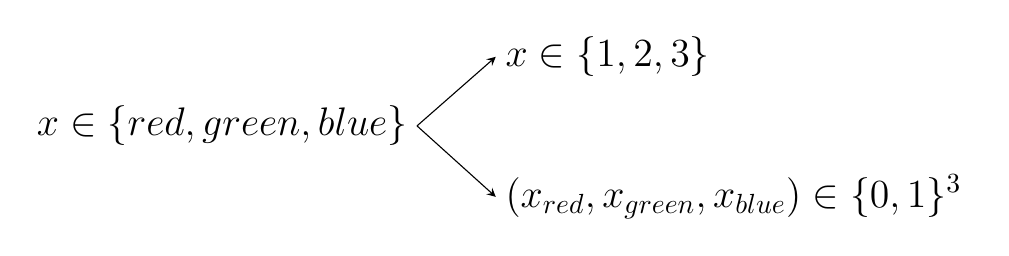
\begin{tikzpicture}[every node/.style={font={\Large}}]
			\onslide<2->{\node[anchor=east] (a) at (0, 0) {$x \in \{ \text{red}, \text{green}, \text{blue} \}$};}
			\onslide<4->{\node[anchor=south west] (b) at (1, .5) {$x \in \{ 1, 2, 3 \}$};}
			\onslide<5->{\node[red!85!black] (bmark) at (b.east) {\quad \huge \xmark};}
			\onslide<8->{
				\node[anchor=north west] (c) at (1,-.5) {$(x_{\text{red}}, x_{\text{green}}, x_{\text{blue}}) \in \{ 0, 1 \}^3$};
				\node[green!75!black] (cmark) at (c.east) {\quad \huge \cmark};
			}
		
			\onslide<4->{\path[-stealth] (a.east) edge (b.west);}
			
			\onslide<8->{\path[-stealth] (a.east) edge (c.west);}
		\end{tikzpicture}
	\end{center}
\end{frame}